% !TEX program = lualatex
\PassOptionsToPackage{table}{xcolor}
\documentclass{matthijs}
\graphicspath{{../assets/}{./docs/assets/}{./docs/functional-design/}}

\begin{filecontents*}[overwrite]{\jobname.xmpdata}
	\Title{Functional Design}
	\Subject{Description of the product}
	\Author{Matthijs Bakker}
	\Language{en-US}
	\Keywords{functional\sep design}
\end{filecontents*}

% BEGIN preamble.tex

% Style for first and last page
\usepackage{wallpaper}
\usepackage{color}
\definecolor{arobsblue}{HTML}{0e335c}

% Versioning plugin that retrieves data from the git repo dir
% Needs the "gitInfoHead" file to be generated, make sure
% that the shim script or the git hook is enabled
\usepackage[maxdepth=2]{gitinfo2}

% Use biblatex with biber backend for bibliography
\usepackage{csquotes}
\usepackage[style=ieee]{biblatex}
\renewcommand*{\mkbibacro}[1]{#1}
\setcounter{biburllcpenalty}{7000}
\setcounter{biburlucpenalty}{8000}

% This lets the text look really juicy
\usepackage{microtype}
\usepackage{extdash}

% A column for right-aligned autowrap text
\newcolumntype{R}{>{\arraybackslash}m{10cm}}

% PDF-A
\usepackage{colorprofiles}
\usepackage[a-3b]{pdfx}
\hypersetup{
	bookmarks=true,
	unicode=false,
	pdftoolbar=true,
	pdfmenubar=true,
	colorlinks=true,
	linkcolor=black,
	citecolor=black,
	filecolor=black,
	urlcolor=black
}
%\hypersetup{
%	colorlinks=true,
%	linkcolor=gray,
%	urlcolor=gray,
%	citecolor=gray
%}

% END preamble.tex


\usepackage{titlepage}

\addbibresource{fd.bib}

\usepackage{tikz}
\usepackage{tikz-uml}
\usetikzlibrary{positioning, arrows.meta}

\usepackage{tabularx}

\begin{document}

	% Set language to English
	\taal{en}

	\maketitlepage{Functional Design}{0.1}
	\pagenumbering{arabic}
	\thispagestyle{empty}
	
	\begin{inhoudspagina}

	\end{inhoudspagina}

	\pagenumbering{arabic}

	\begin{hoofdstuk}{Preface}

		The functional design consists of the requirements and expectations of the end product.
		It is a way to establish that the product meets the demands that were assigned to it.
		The requirements are framed from the perspective of the users and stakeholders to give background on why they need to be implemented.

		\bigskip

		Furthermore, a general high-level overview of the system is given to show where it will be integrated in the total picture.

	\end{hoofdstuk}

	\begin{hoofdstuk}{System Overview}

		To give a total picture of the system and where it should be integrated with existing systems, an overview graphic is provided which gives a visual representation of the situation.
		The information flow between the parts of the system is visualized by arrows.
		These arrows are accompanied by labels which describe the type of information that is passed on.

		\vspace{4ex}

		\begin{figuur}{A high-level overview of the system integration}

			\begin{tikzpicture}

				\node[inner sep=0] (fpga) {
					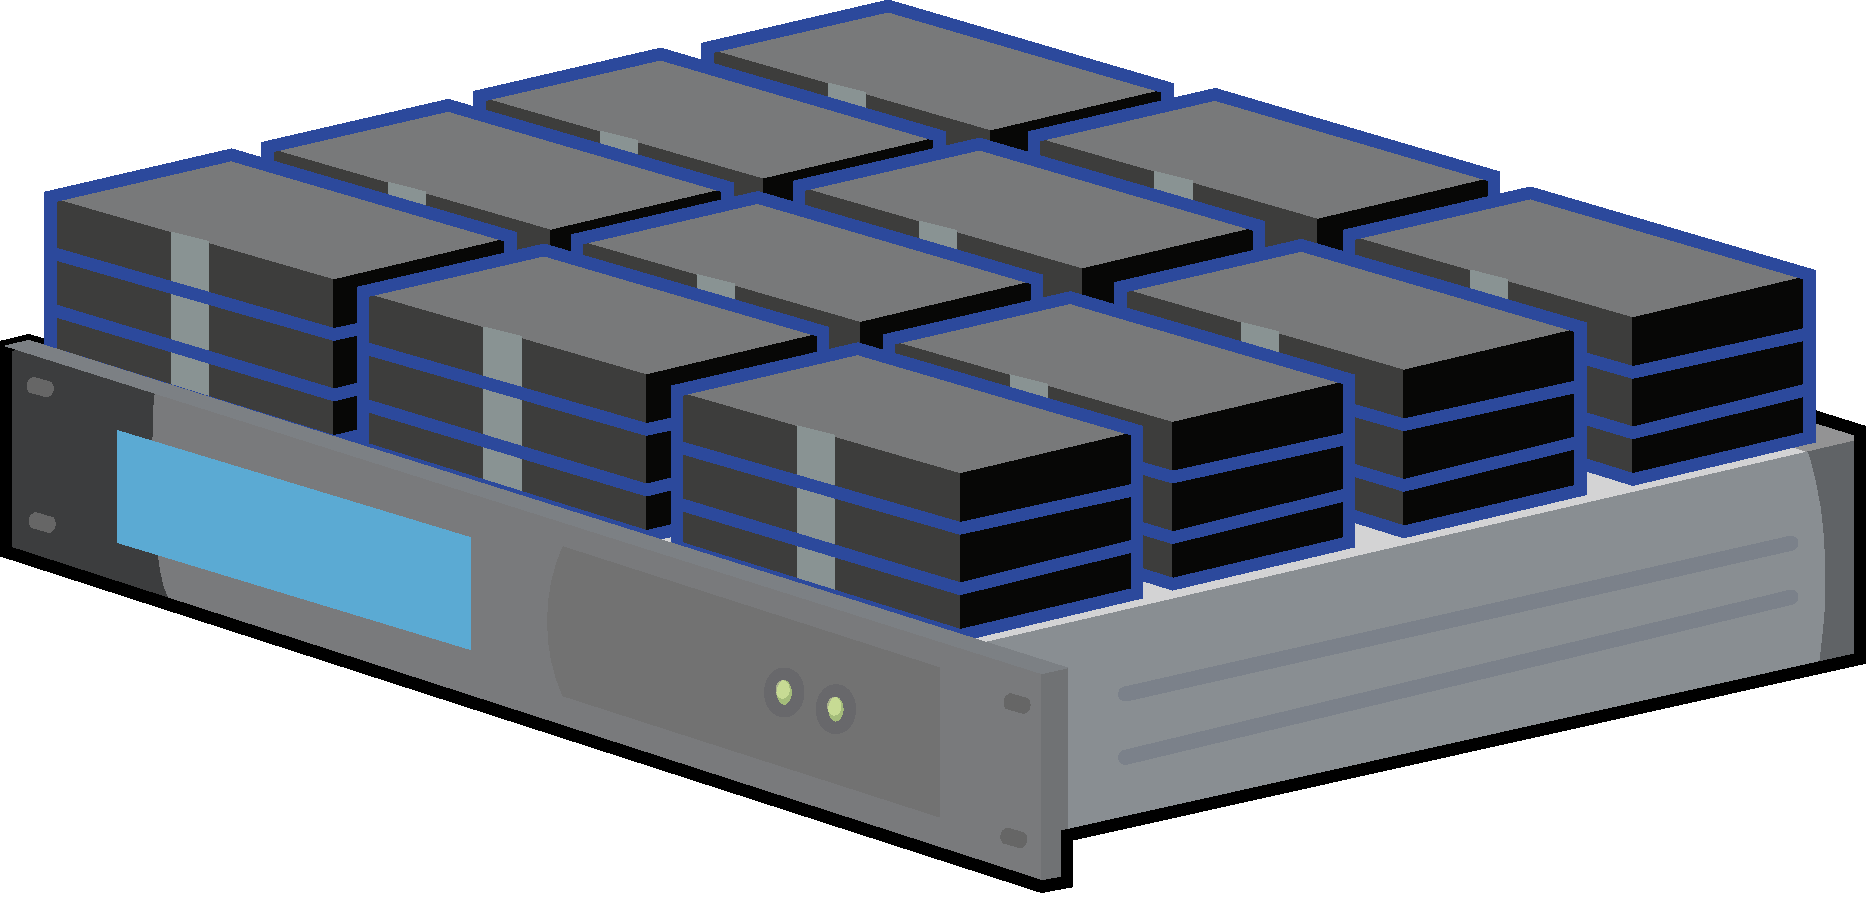
\includegraphics[width=0.2\textwidth]{asset_csdx_netscaler.pdf}
				};
				\node[anchor=south, above=1ex of fpga, align=center, inner sep=0] (fpga label) {FPGA Accelerated\\Vision Processing Unit};

				\node[inner sep=1ex, below left=8ex and 18ex of fpga] (camera) {
					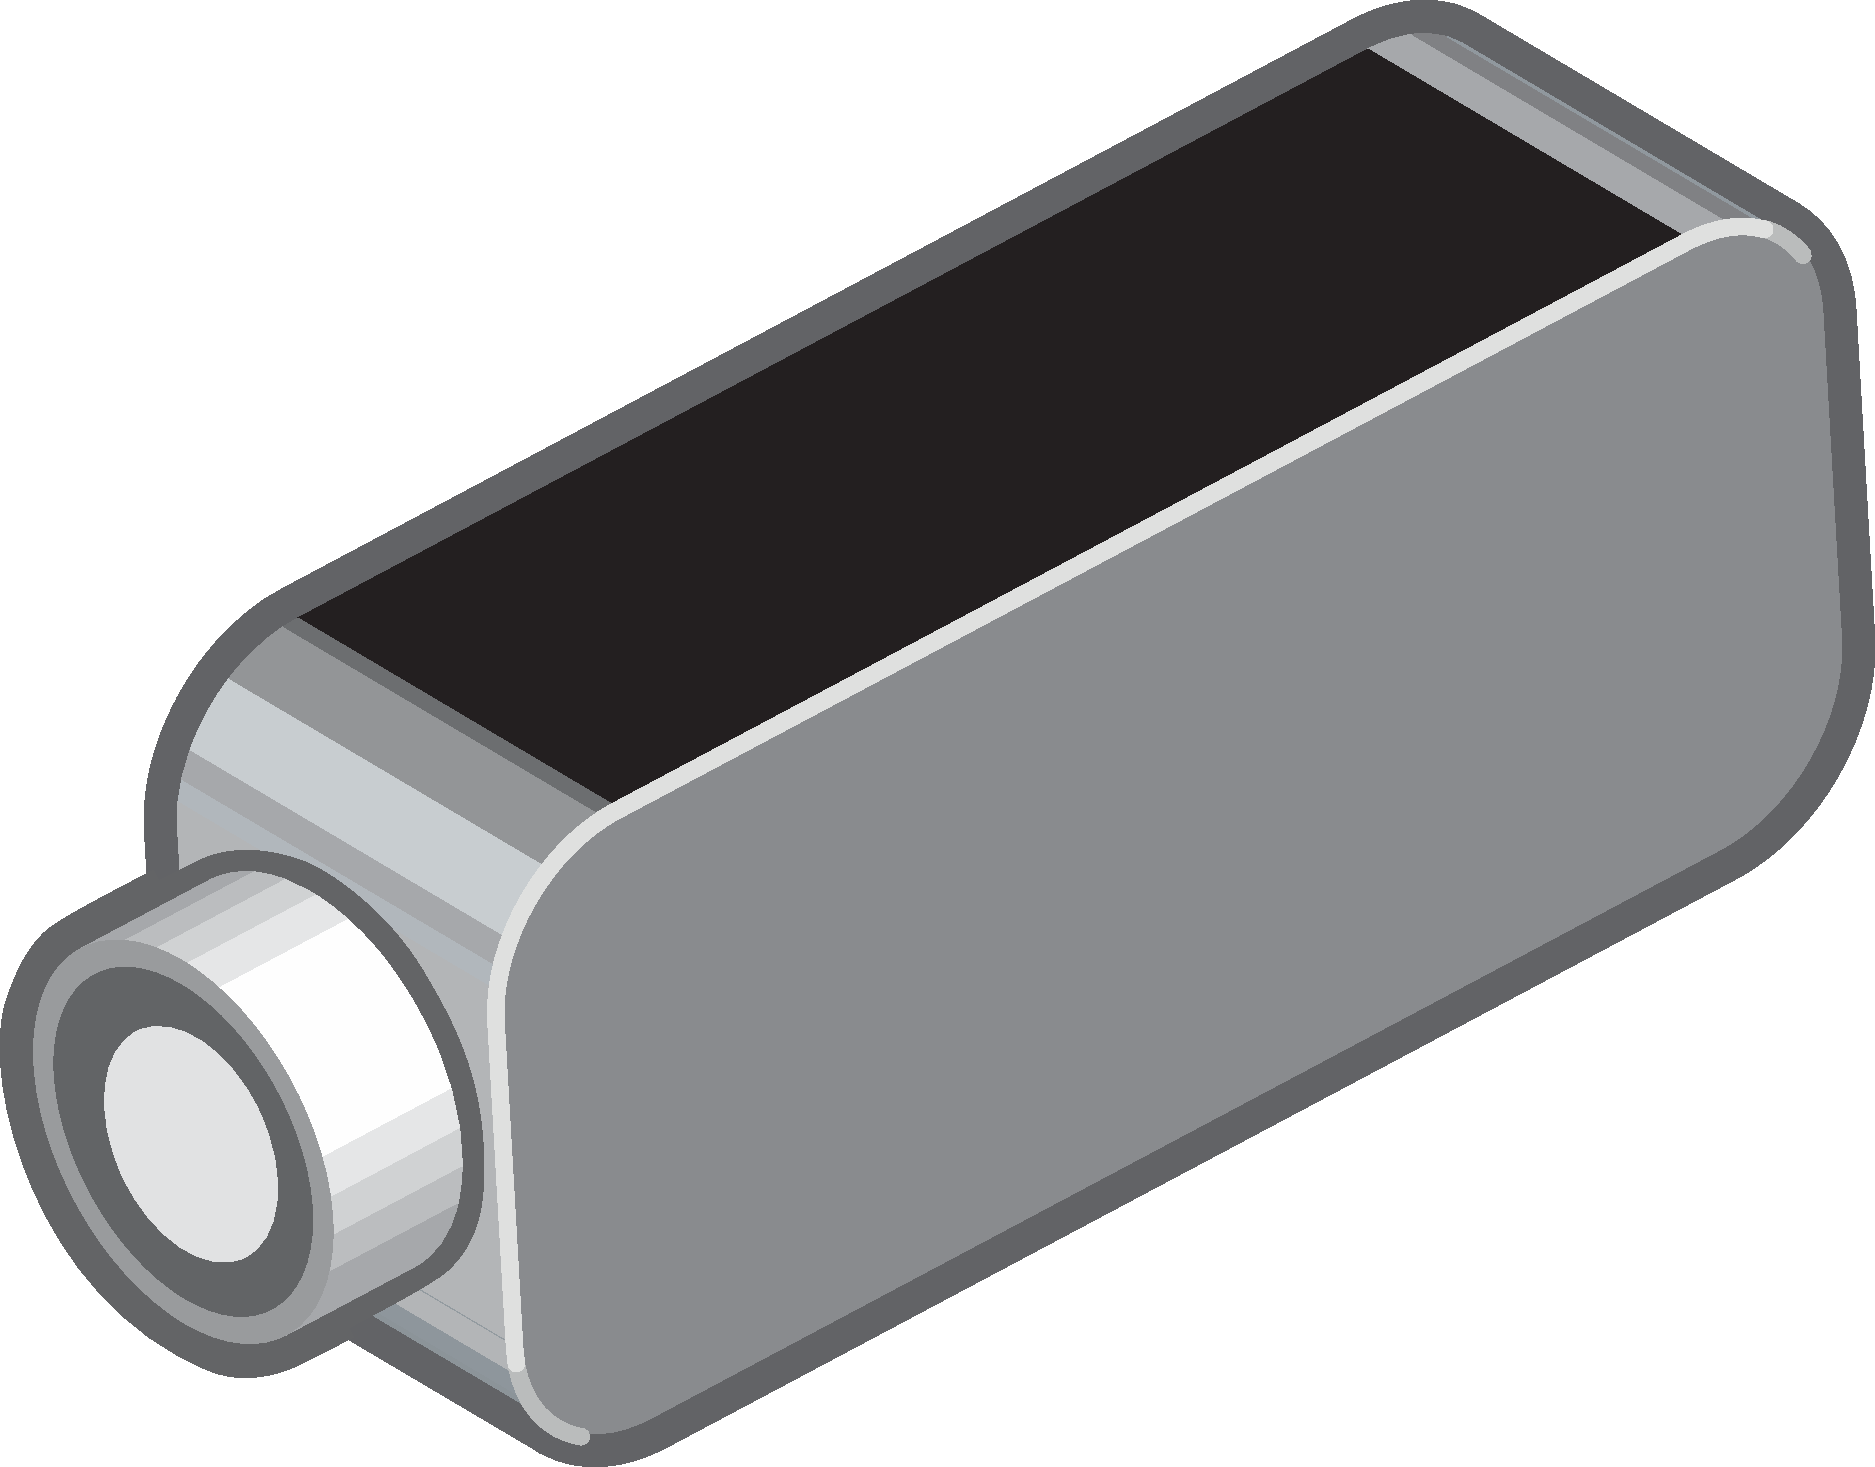
\includegraphics[width=0.1\textwidth]{asset_csdx_camera.pdf}
				};
				\node[anchor=south, above=0.5ex of camera, align=center, inner sep=0] (camera label) {Dashboard\\Camera};
				
				\node[inner sep=1ex, below right=8ex and 18ex of fpga] (ldws) {
					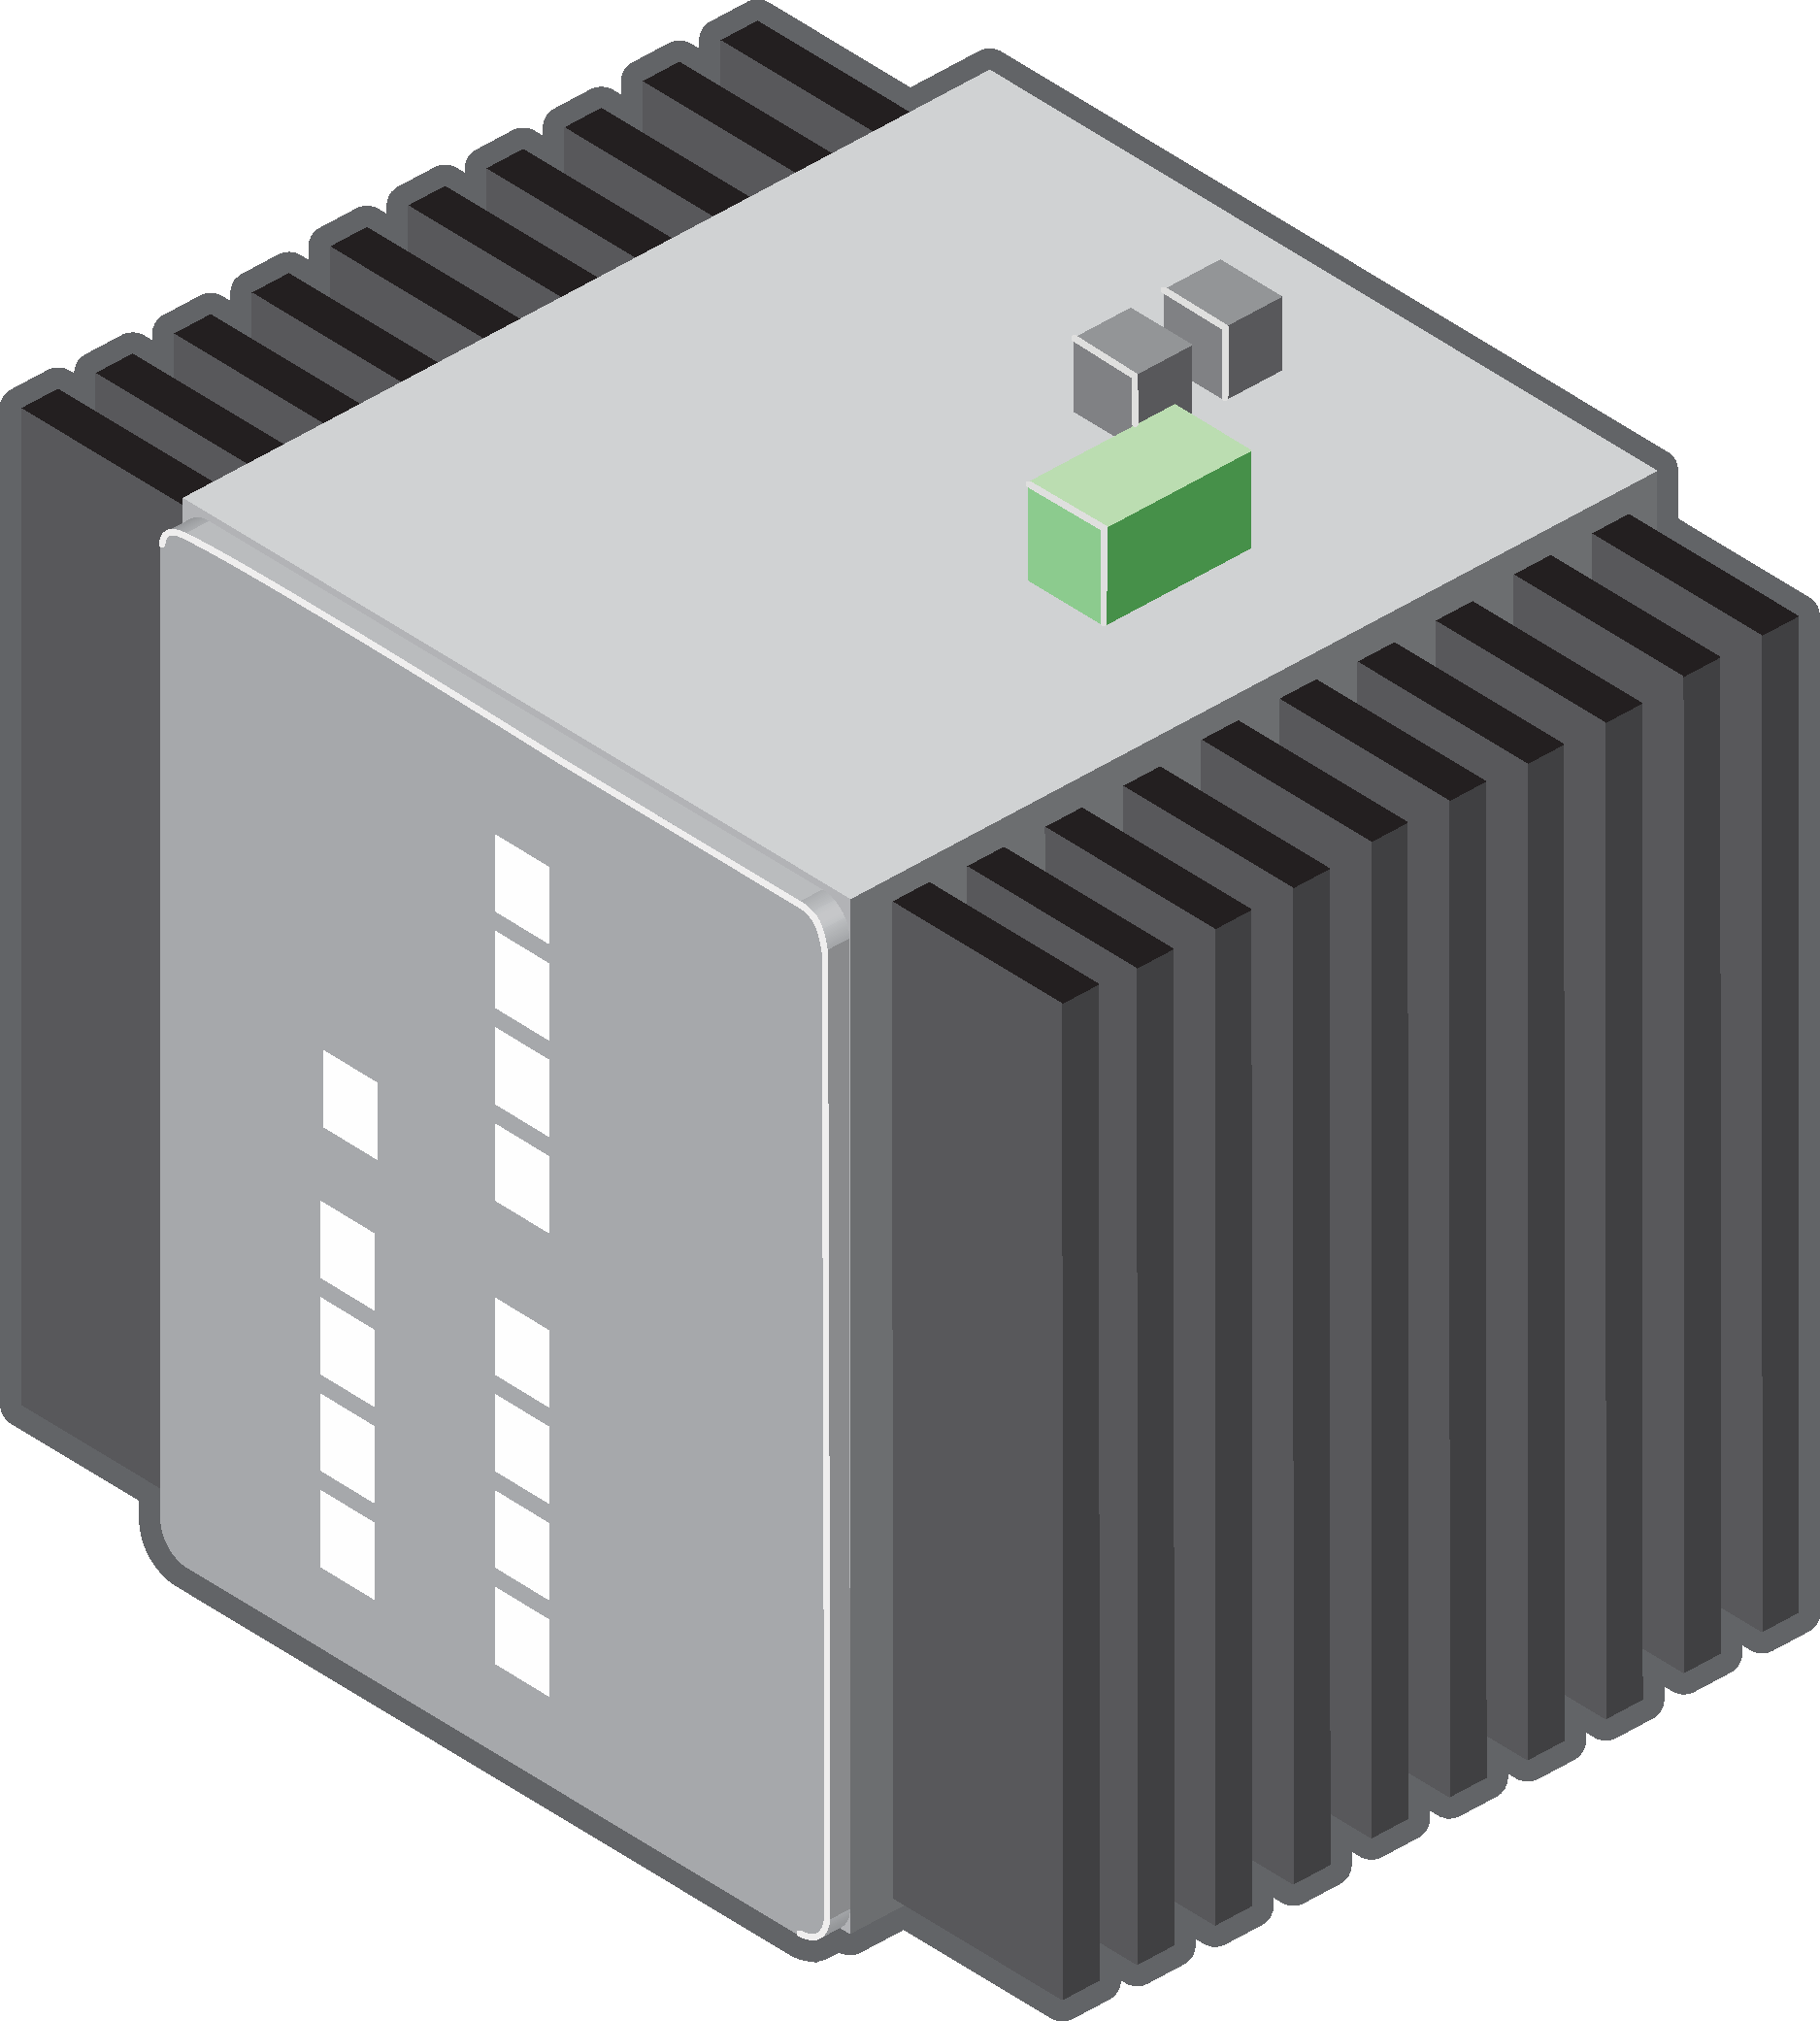
\includegraphics[width=0.1\textwidth]{asset_csdx_switch.pdf}
				};
				\node[anchor=south, above=0.5ex of ldws, align=center, inner sep=0] (ldws label) {Lane Departure\\Warning System};

				\node[below=22ex of fpga, align=center, inner sep=0, xshift=1ex] (info) {
						(graphics used from the Allied Telesis stencil set \cite{allied2014stencils})
				};

				\draw [-{Latex[length=5pt, width=5pt]}] (camera) -- (fpga) node [pos=.5, above, sloped] (camera fpga label) {\small video stream};;
				\draw [-{Latex[length=5pt, width=5pt]}] (fpga) -- (ldws) node [pos=.5, above, sloped] (fpga ldws label) {\small lane params};;

			\end{tikzpicture}

			\vspace{-1.5ex}

		\end{figuur}

		It is assumed that the dashcam and the Lane Departure Warning System (LDWS) already exist in the context of the car.
		This project will only focus on the research and development of the Vision Processing Unit (VPU).
		The dashcam is an OV7670 camera module which will be connected to the VPU to provide a video stream from the front perspective of a vehicle.
		The LDWS is a subsystem of the Advanced Driver-Assistance System (ADAS) which will trigger certain actions based on observations made by arbitrary business logic on the basis of the lane parameter data.
		This lane parameter data consists of information which can be used to determine whether the car is driving in the lane or not.
		Deciding which actions take place in the LDWS is out of scope of this project.

	\end{hoofdstuk}

	\begin{hoofdstuk}{Requirements}

		A user story is a requirement that is viewed from the perspective of a user or stakeholder.
		This story helps to identify what a certain person expects from the product and why he expects it.
		Each story is made concrete and measurable by acceptance criteria to guarantee that the product meets the goal of the user.

		\bigskip

		A product quality category from the ISO/IEC 25010:2011 standard \cite{iso25010systems} has been assigned to every user story and is represented in italic text in the enumeration below.

		\vspace{1ex}

		\begin{figuur}{User Stories}

			\begin{enumerate}[labelsep=2ex, font=\bfseries]
				
				\item	As the production company I want to be able to produce the lane detection system as economically as possible

					\begin{enumerate}[leftmargin=8ex]

						\item	The system is formally verified and implemented on an FPGA -- \textit{Maturity}
						\item	Faulty systems can be fixed by only replacing the FPGA -- \textit{Replaceability}
						\item	The digital logic layer is compact enough to fit on the Artix 7 XC7A35T chip family -- \textit{Resource utilization}
						\item	The system interacts with the existing OV7670 camera module -- \textit{Adaptability}

					\end{enumerate}

				\item	As a systems integrator I want to be able to integrate the lane detection system into existing Advanced Driver-Assistance Systems

					\begin{enumerate}[leftmargin=8ex]

						\item	Up-to-date technical documentation is provided which explains how the lane detection system interacts with other automobile systems -- \textit{Maintainability}
						\item	The protocols used to communicate with other automobile systems are documented -- \textit{Maintainability}
						\item	The system can be integrated into other ecosystems -- \textit{Reusability \& adaptability}

					\end{enumerate}

				\item	As an automobile technician I want to be able to troubleshoot issues with the lane detection system when repairing vehicles

					\begin{enumerate}[leftmargin=8ex]

						\item	The system can be debugged using a laptop -- \textit{Maintainability}
						\item	The resulting video feed can be extracted in real-time -- \textit{Analysability}
						\item	The resulting lane parameters can be extracted in real-time -- \textit{Analysability}

					\end{enumerate}

				\item	As a vehicle driver I want my vehicle to warn me in real-time if I'm about to leave the road lane

					\begin{enumerate}[leftmargin=8ex]

						\item The lane detection system can operate on the camera video feed in \mbox{real-time -- \textit{Availability}}
						\item The latency of the lane detection system is shorter than the time between the frames of the camera feed -- \textit{Time behavior}

					\end{enumerate}

			\end{enumerate}

		\end{figuur}

	\end{hoofdstuk}

	\begin{hoofdstuk}{Use Cases}

		An illustration of the actions of the system's components and the relationships with external components can be seen in \verwijzingb{figuur}{Use case diagram}.
		Human actors as well as system actors are modelled in this illustration.

		\vspace{2ex}

		\begin{figuur}{Use case diagram}

			\begin{tikzpicture}

				\begin{umlsystem}[x=4, fill=arobsblue!5]{Lane Detection System}
					\umlusecase[alias=cv, x=3]{Capture video}
					\umlusecase[alias=dl, y=-2,x=0.25]{Detect lane}
					\umlusecase[alias=pv, x=6, y=-2, fill=yellow!20]{Process video}
					
					\umlusecase[alias=cl, x=0.5, y=-4]{Calculate position}
					\umlusecase[draw=none, fill=none, y=-5.5]{} %phantom to extend system
				\end{umlsystem}

				\umlactor[x=0,y=-2]{Video Unit}
				\umlactor[x=14]{Dashcam}
				\umlactor[x=14,y=-3]{Technician}
				\umlactor[x=14,y=-6]{LDWS}

				\umlassoc{Dashcam}{cv}
				\umlassoc[stereo=use]{Video Unit}{cv}
				\umlassoc{Video Unit}{dl}
				\umlassoc{Video Unit}{cl}
				\umlassoc[stereo=use]{Technician}{pv}
				\umlassoc[stereo=use]{Technician}{cl}
				\umlassoc[stereo=use]{cl}{LDWS}

				\umlinclude{cv}{pv}
				\umlinclude{dl}{pv}

			\end{tikzpicture}

			\vspace{-3ex}

		\end{figuur}

	\end{hoofdstuk}

	\begin{hoofdstuk}{User Interface Design}

		The troubleshooting application for automobile technicians will have a simple GUI frontend which will display a read-out of the algorithm values.
		It will also have a preview screen where detected lane lines are plotted.
		A lane departure warning status must be shown to indicate if an upcoming lane departure is predicted.

		\bigskip

		The following elements must be visible on the user interface in order to satisfy technicians:

		\begin{enumerate}

			\item The values of the parameters used in the video processing lane detection algoritm
			\item A simulated preview of the lane lines which were detected
			\item Whether or not a departure is currently detected based on the results of the plotted lines

		\end{enumerate}

		\bigskip

		\centerline{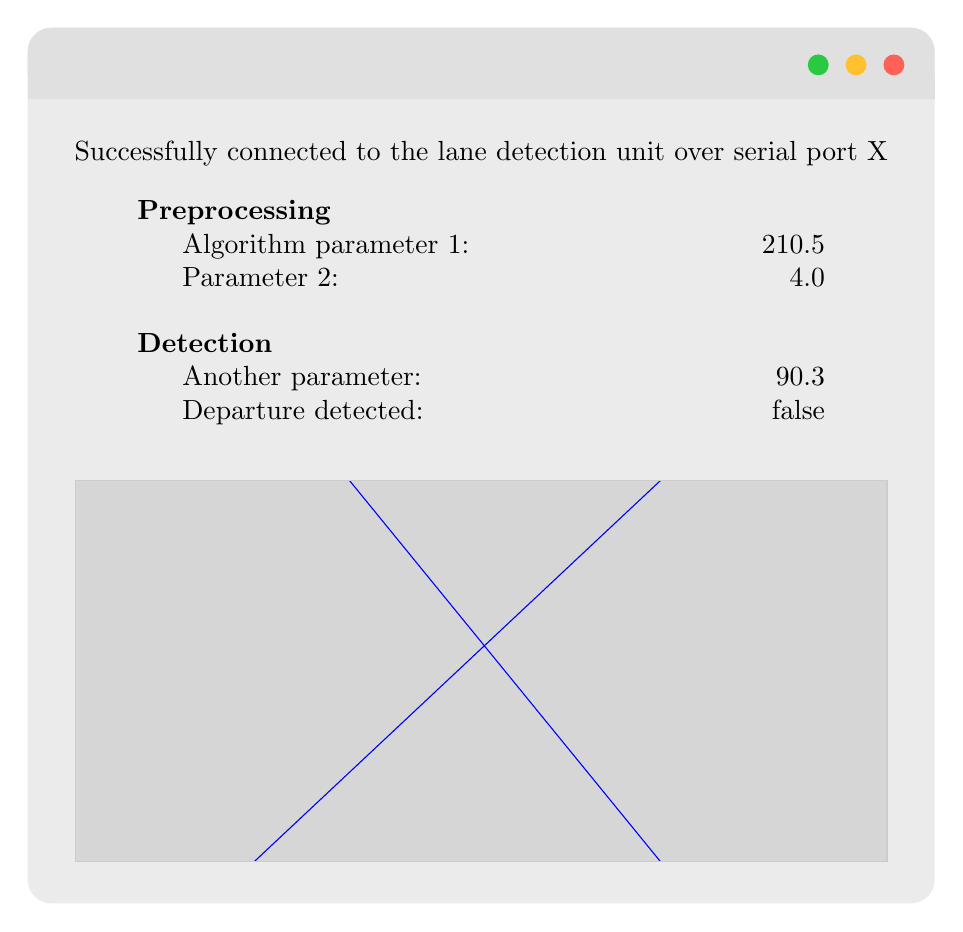
\begin{tikzpicture}

			% This looks so freaking good...
			% I don't like Apple but they do have god tier designers

			\definecolor{osx-red}{HTML}{ff6159}
			\definecolor{osx-yellow}{HTML}{ffc12e}
			\definecolor{osx-green}{HTML}{28ca42}

			\node (bg) [draw=none, fill=black!8, rounded corners=2ex, minimum width=.95\textwidth, minimum height=73.5ex] at (0,0) {};

			% top bar
			\node (top bar) [draw=none, fill=black!12, rounded corners=2ex, minimum width=.95\textwidth, minimum height=6ex, anchor=north] at (bg.north) {};
			\node (top bar nocornerssouth) [draw=none, fill=black!12, minimum width=.95\textwidth, minimum height=2ex, anchor=south] at (top bar.south) {};
			\node (btn exit) [fill=osx-red, circle, inner sep=0pt, outer sep=0pt, anchor=center, minimum size=1.75ex, below left=2.55ex and 2.85ex of top bar.north east] {};
			\node (btn min) [fill=osx-yellow, circle, inner sep=0pt, outer sep=0pt, anchor=center, minimum size=1.75ex, below left=2.55ex and 6.025ex of top bar.north east] {};
			\node (btn max) [fill=osx-green, circle, inner sep=0pt, outer sep=0pt, anchor=center, minimum size=1.75ex, below left=2.55ex and 9.2ex of top bar.north east] {};


			\node (details) [fill=none, minimum width=.85\textwidth, minimum height=20ex, anchor=north, below=3.5ex of top bar.south, align=center, text depth=20ex, inner sep=0, outer sep=0] {
				Successfully connected to the lane detection unit over serial port X \\
				\\
				\begin{tabularx}{0.755\linewidth}{X r}
					\textbf{Preprocessing} & \tabularnewline
					% yes, 3 space tabs,,,,,,,,,
					\hspace{3ex} Algorithm parameter 1: & 210.5 \tabularnewline
					\hspace{3ex} Parameter 2: & 4.0 \tabularnewline
					& \tabularnewline
					\textbf{Detection} & \tabularnewline
					\hspace{3ex} Another parameter: & 90.3 \tabularnewline
					\hspace{3ex} Departure detected: & false \tabularnewline
				\end{tabularx}
			};

			% I love tikz so much
			\node (preview) [draw=black!20, fill=black!16, minimum width=.85\textwidth, minimum height=32ex, anchor=south, above=3.5ex of bg.south, path picture={
				\draw[blue] ([xshift=23ex]path picture bounding box.north west) -- ([xshift=-19ex]path picture bounding box.south east);
				\draw[blue] ([xshift=-19ex]path picture bounding box.north east) -- ([xshift=15ex]path picture bounding box.south west);
			}] {};

		\end{tikzpicture}}

	\end{hoofdstuk}

	% Bibliography page
	\begin{hoofdstuk}{References}

		\printbibliography[heading=none]

	\end{hoofdstuk}

	\makelastpage

\end{document}
